\subsection{Introducción a las excepciones}
En Python, las excepciones son eventos inesperados o errores que ocurren durante la ejecución de un programa. Estos errores pueden ser causados por diversas situaciones, como divisiones por cero, acceso a archivos inexistentes o intentos de acceder a índices fuera de rango en listas. En resumen, Python nos proporciona una estructura para manejar estas excepciones y evitar que el programa se detenga abruptamente.

\subsection{Uso de try, except, else}
\begin{itemize}
    \item Try: El bloque ``try'' se utiliza para envolver el código en el que esperas que ocurra una excepción. Dentro de este bloque, colocas el código que podría generar una excepción. Si una excepción se produce en el bloque ``try'', el flujo de control se traslada al bloque ``except''.
    \item Except: El bloque ``except'' se utiliza para manejar excepciones. Puedes especificar el tipo de excepción que deseas capturar después de la palabra clave ``except''. Si ocurre una excepción del tipo especificado en el bloque try, se ejecutará el código en el bloque ``except''. Puedes tener varios bloques ``except'' para manejar diferentes tipos de excepciones.
    \begin{figure}[h]
        \centering
        \scalebox{0.35}{
        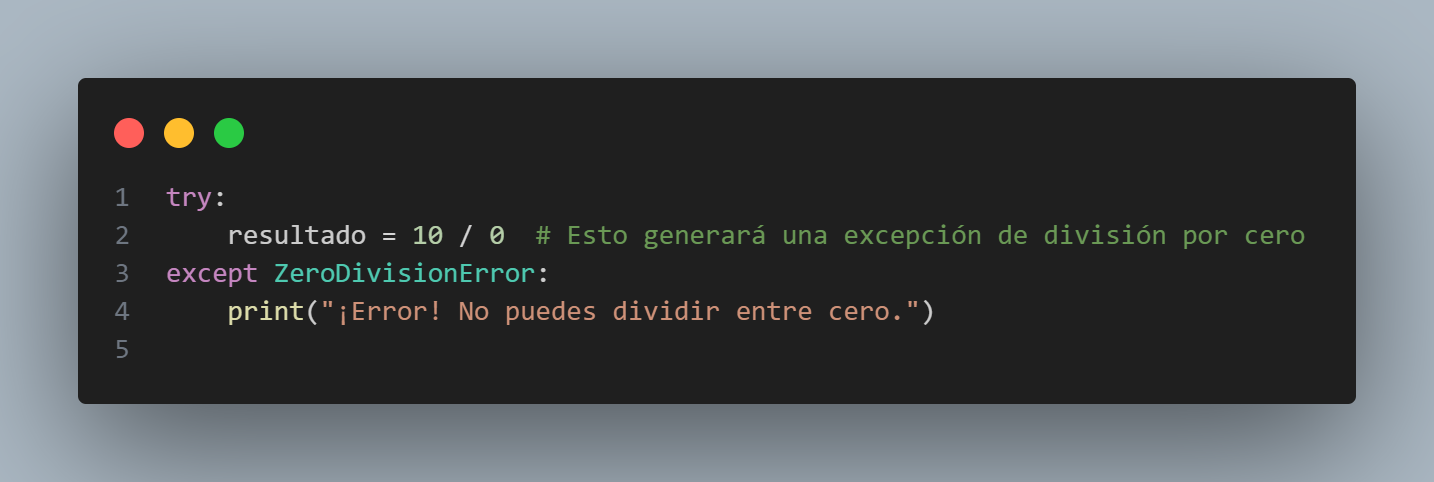
\includegraphics{Imagenes/manejo1.png}
        }
      \end{figure}
    
    
    \item Else: El bloque ``else'' es opcional y se coloca después de todos los bloques ``except''. Se ejecuta si no se ha producido ninguna excepción en el bloque ``try''. Es útil para ejecutar código que debe ejecutarse solo si no se generan excepciones.
    \begin{figure}[h]
        \centering
        \scalebox{0.35}{
        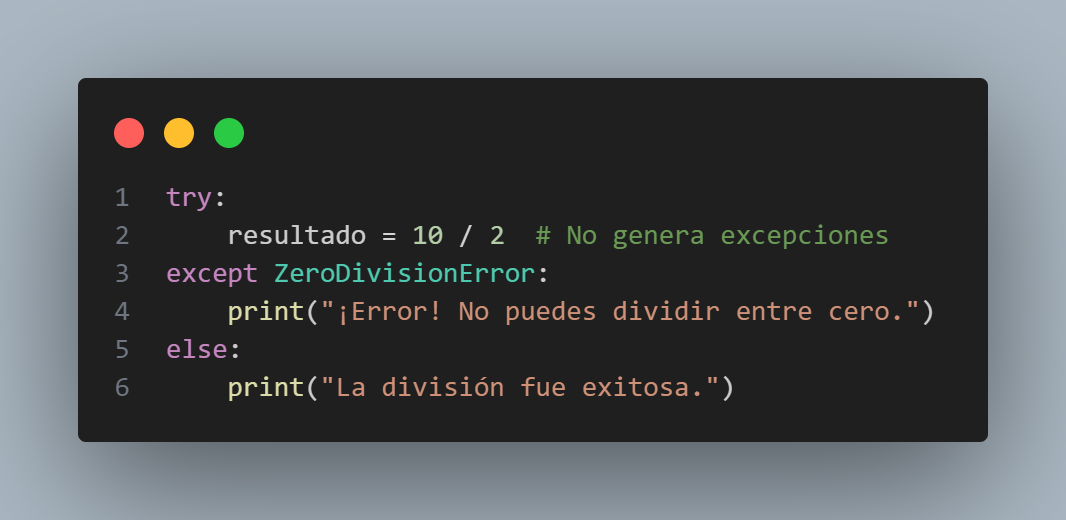
\includegraphics{Imagenes/manejo2.png}
        }
      \end{figure}
    
    \item Finally: El bloque ``finally'' es opcional y se coloca al final, después de todos los bloques ``except'' y, si se utiliza, después del bloque ``else''. El código en este bloque se ejecuta sin importar si se produjo una excepción o no. Se utiliza comúnmente para realizar la limpieza de recursos, como cerrar archivos o conexiones de bases de datos, garantizando que se realicen incluso en caso de excepciones.
    \begin{figure}[h]
        \centering
        \scalebox{0.35}{
        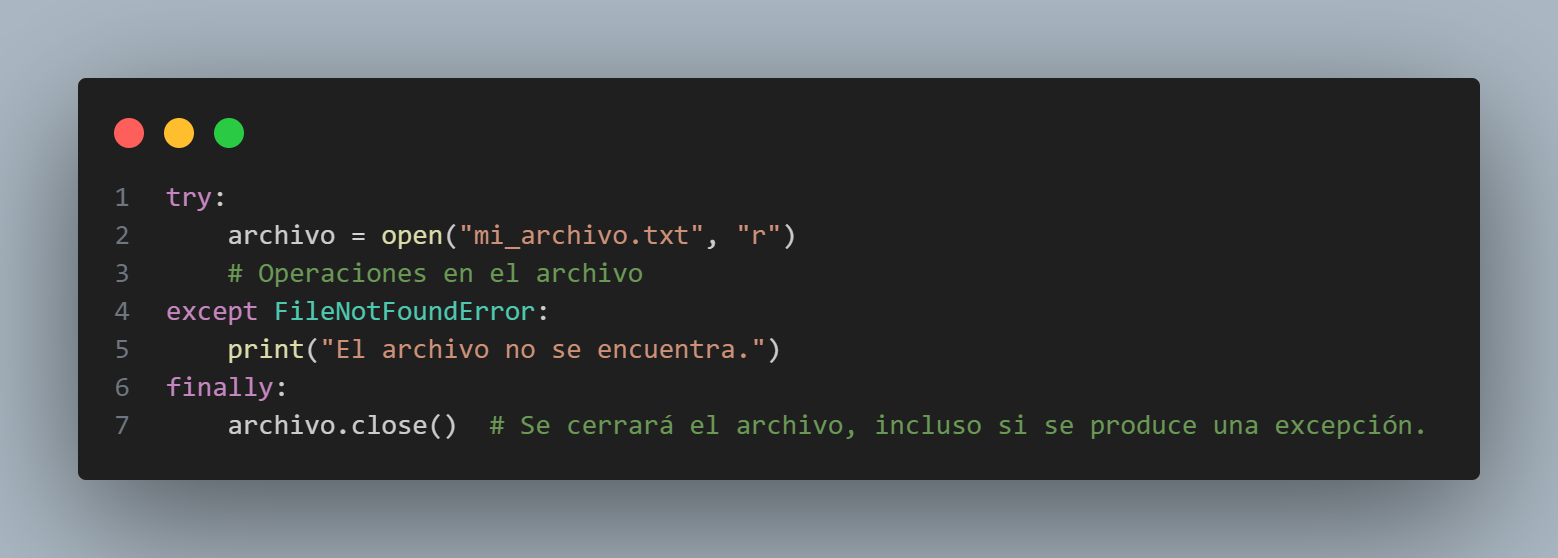
\includegraphics{Imagenes/manejo3.png}
        }
      \end{figure}

\end{itemize}

\subsection{Tipos de excepciones y manejo específico}
\begin{itemize}
    \item ZeroDivisionError: Se genera cuando intentas dividir un número entre cero.
    \begin{figure}[h]
        \centering
        \scalebox{0.35}{
        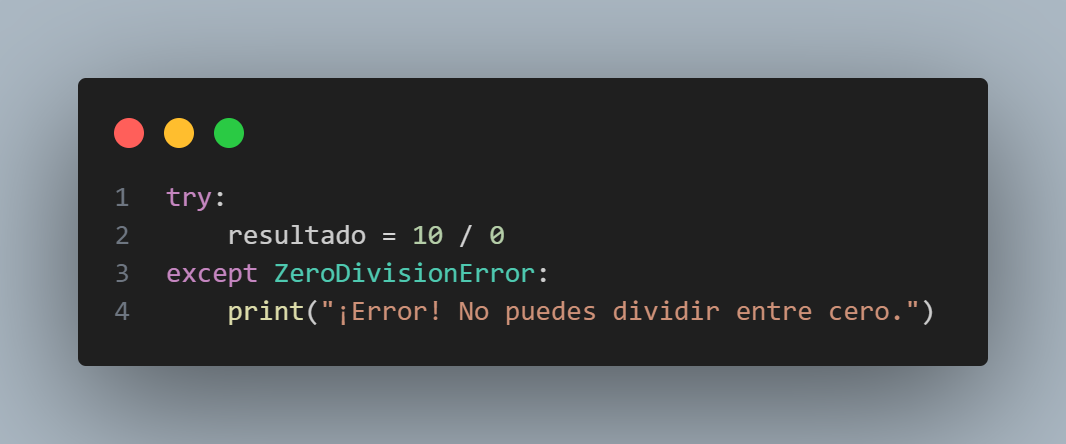
\includegraphics{Imagenes/manejo4.png}
        }
      \end{figure}
    \newpage
    \item FileNotFoundError: Ocurre cuando intentas abrir o realizar operaciones en un archivo que no existe.
    \begin{figure}[h]
        \centering
        \scalebox{0.35}{
        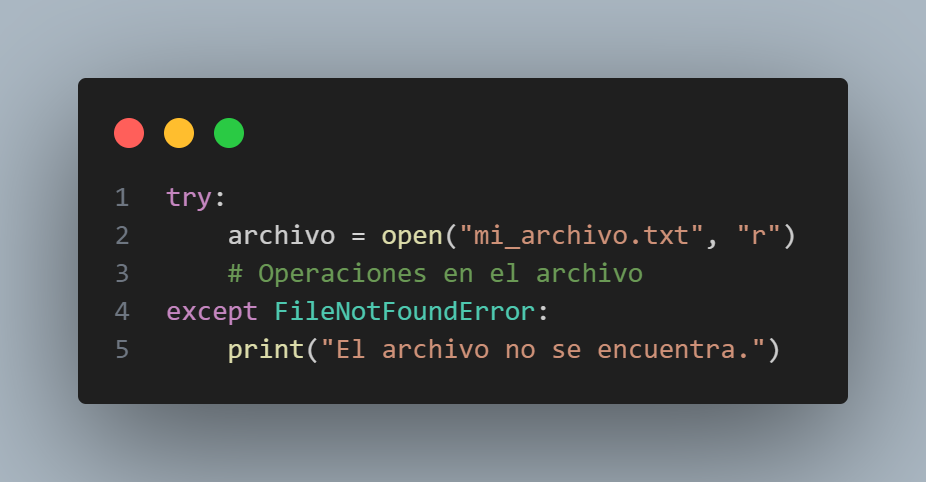
\includegraphics{Imagenes/manejo5.png}
        }
      \end{figure}
    
    \item TypeError: Esta excepción se produce cuando realizas una operación en un tipo de dato que no es compatible.
    \begin{figure}[h]
        \centering
        \scalebox{0.35}{
        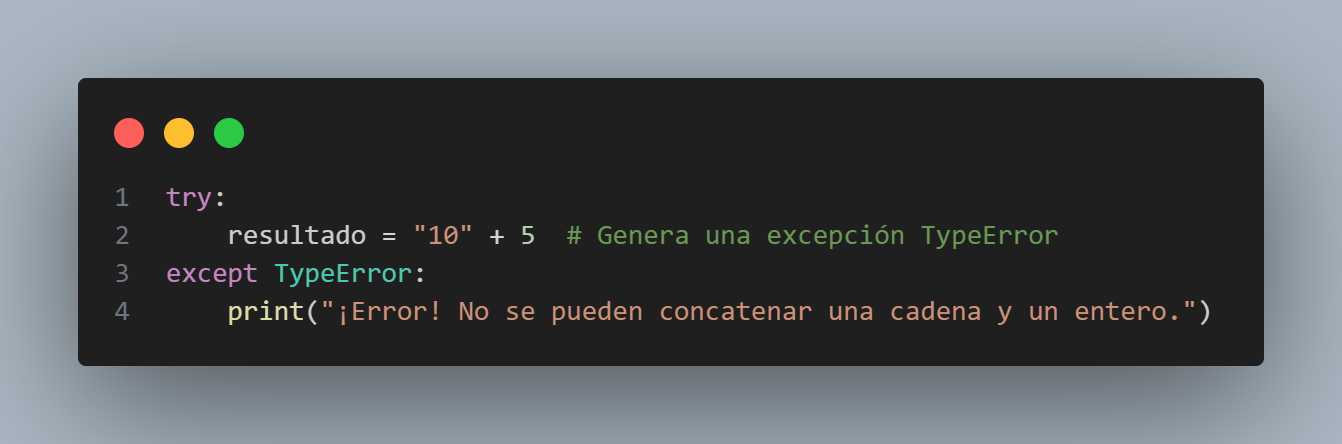
\includegraphics{Imagenes/manejo6.png}
        }
      \end{figure}
    
    
    \item IndexError: Se genera al intentar acceder a un índice fuera de rango en una lista o secuencia.
    \begin{figure}[h]
        \centering
        \scalebox{0.35}{
        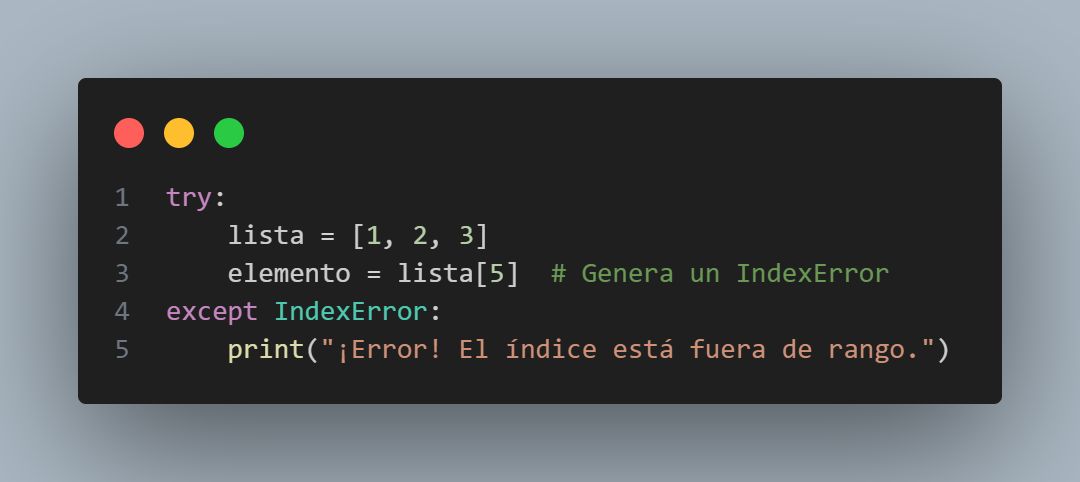
\includegraphics{Imagenes/manejo7.png}
        }
      \end{figure}
    
    
    \item ValueError: Esta excepción ocurre cuando el tipo de dato es correcto, pero el valor no es válido para la operación.
    \begin{figure}[h]
        \centering
        \scalebox{0.35}{
        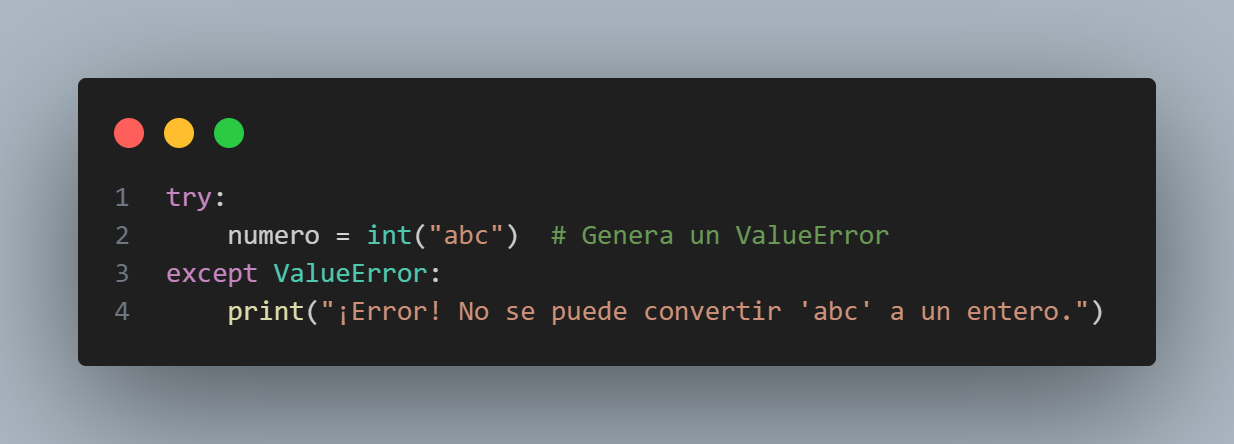
\includegraphics{Imagenes/manejo8.png}
        }
      \end{figure}
    
    \item Custom Exceptions: Además de las excepciones incorporadas, puedes crear tus propias excepciones personalizadas extendiendo la clase Exception. Esto es útil cuando deseas manejar situaciones específicas en tu programa.
    \begin{figure}[h]
        \centering
        \scalebox{0.35}{
        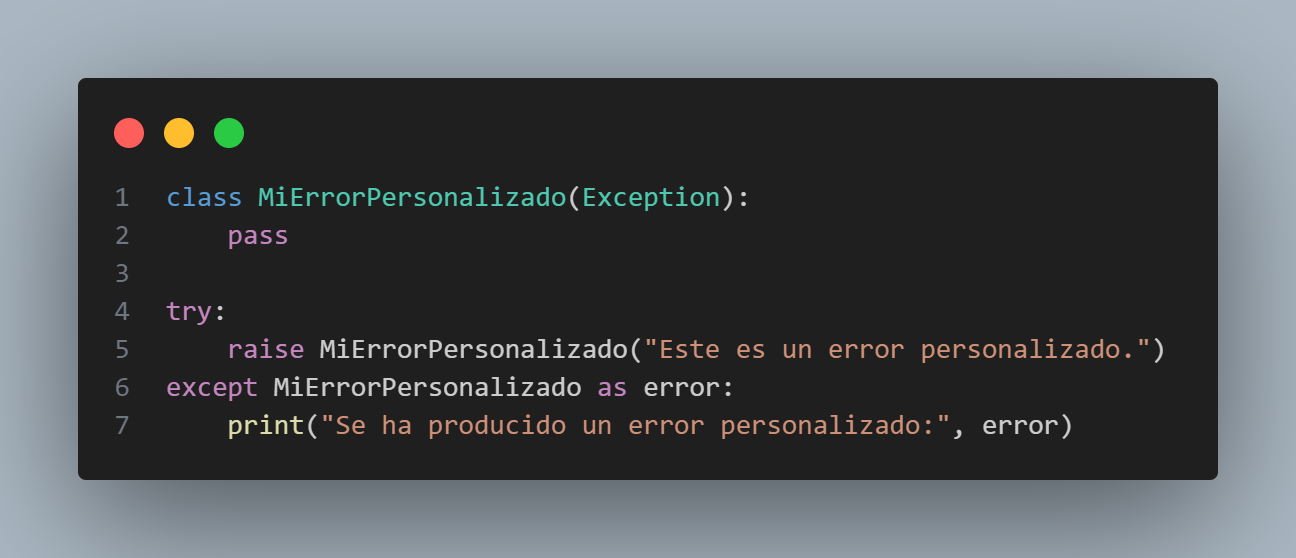
\includegraphics{Imagenes/manejo9.png}
        }
      \end{figure}
    

\end{itemize}
